\documentclass[t,18pt]{beamer}
\usepackage[utf8]{inputenc}
\usepackage{graphbox}

\usetheme{Rochester}

\newcommand{\emdash}{---}
\newcommand{\etal}[0]{et al.\@}
\newcommand{\light}[1]{\textcolor{black!40}{#1}}

\setbeamercolor{normal text}{fg=black}
\setbeamercolor{frametitle}{fg=white}

\makeatletter
\setbeamertemplate{footline}
{
  \leavevmode%
  \hbox{%
  \begin{beamercolorbox}[wd=.5\paperwidth,ht=2.25ex,dp=1ex,center]{author in head/foot}%
    \usebeamerfont{author in head/foot}\insertshortauthor
  \end{beamercolorbox}%
  \begin{beamercolorbox}[wd=.5\paperwidth,ht=2.25ex,dp=1ex,right]{date in head/foot}%
    \usebeamerfont{date in head/foot}\insertshortdate{}\hspace*{2em}
    \insertframenumber{} / \inserttotalframenumber\hspace*{2ex}
  \end{beamercolorbox}}%
  \vskip0pt%
}
\makeatother



% TODO: Maybe drop evaluation and only show examples?


\begin{document}

\title{Visualizing Dynamic Clustered Data Using Area-proportional Maps}
\author{Christian Schnorr}

\begin{frame}
  \titlepage
\end{frame}





\section{Introduction}
\label{sect:introduction}

\begin{frame}
  \frametitle{Agenda}
  \begin{itemize}
    \item \nameref{sect:introduction} \begin{itemize}
      \item \nameref{subsect:problem-statement}
      \item \nameref{subsect:motivation}
    \end{itemize}
    \item \light{\nameref{sect:visualizing-static-input-graphs}}
    \item \light{\nameref{sect:visualizing-dynamic-input-graphs}}
    \item \light{\nameref{sect:evaluation}}
  \end{itemize}
\end{frame}

\subsection{Problem Statement}
\label{subsect:problem-statement}

\begin{frame}
  \frametitle{\nameref{subsect:problem-statement}}
  \begin{itemize}
    \item Visualize clustered graph as a map \begin{itemize}
      \item Each country represents a cluster in the original graph
      \item Countries have area close to proportional to cluster size
      \item Dynamic setting: input graph changes over time $\to$ map needs to adapt
    \end{itemize}
    \begin{figure}
      \includegraphics[height=2.2cm]{../Thesis/Resources/Evaluation-Example-Dynamics-AE097F3A-14FD-4735-A19B-8FD343CA3346-0.pdf}
      \includegraphics[height=2.2cm]{../Thesis/Resources/Evaluation-Example-Dynamics-AE097F3A-14FD-4735-A19B-8FD343CA3346-1.pdf}
      \includegraphics[height=2.2cm]{../Thesis/Resources/Evaluation-Example-Dynamics-AE097F3A-14FD-4735-A19B-8FD343CA3346-2.pdf}
      \includegraphics[height=2.2cm]{../Thesis/Resources/Evaluation-Example-Dynamics-AE097F3A-14FD-4735-A19B-8FD343CA3346-3.pdf}
    \end{figure}
  \end{itemize}
\end{frame}

\subsection{Motivation}
\label{subsect:motivation}

\begin{frame}
  \frametitle{\nameref{subsect:motivation}}
  \begin{itemize}
    \item Clustered data appears naturally
    \item Map metaphor helps us make sense of data
    \item Dynamic data appears naturally: preserving mental map is crucial
    \item Area is a strong visual variable
  \end{itemize}
\end{frame}





\section{Visualizing Static Input Graphs}
\label{sect:visualizing-static-input-graphs}

\begin{frame}
  \frametitle{Agenda}
  \begin{itemize}
    \item \light{\nameref{sect:introduction}}
    \item \nameref{sect:visualizing-static-input-graphs} \begin{itemize}
      \item \nameref{subsect:definitions}
      \item \nameref{subsect:algorithmic-pipeline-static}
      \item \nameref{subsect:transformation-to-dual}
      \item \nameref{subsect:drawing-the-polygonal-dual}
    \end{itemize}
    \item \light{\nameref{sect:visualizing-dynamic-input-graphs}}
    \item \light{\nameref{sect:evaluation}}
  \end{itemize}
\end{frame}

\subsection{Definitions}
\label{subsect:definitions}

\begin{frame}
  \frametitle{\nameref{subsect:definitions}}
  \begin{itemize}
    \item Polygonal contact representation \begin{itemize}
      \item Contact representation in which all regions are simple polygons
      \item No holes
      \item No duplicate adjacencies
    \end{itemize}
    \item Polygonal dual of graph G \begin{itemize}
      \item Polygonal contact representation of G
    \end{itemize}
  \end{itemize}
  \begin{figure}
    \includegraphics[align=c,height=3cm]{../Thesis/Resources/Transformation-Algorithm-1.pdf}\quad
    \includegraphics[align=c,height=3cm]{../Thesis/Resources/Transformation-Algorithm-3.pdf}
  \end{figure}
\end{frame}

\subsection{Algorithmic Pipeline}
\label{subsect:algorithmic-pipeline-static}

\begin{frame}[c]
  \frametitle{\nameref{subsect:algorithmic-pipeline-static}}
  \begin{figure}
    \includegraphics[width=\textwidth]{../Thesis/Resources/Framework-1.pdf}
  \end{figure}
\end{frame}

\subsection{Transformation to Dual}
\label{subsect:transformation-to-dual}

\begin{frame}[c]
  \frametitle{\nameref{subsect:transformation-to-dual}}
  \framesubtitle{Definition: Augmented Dual $G^+$}
  \begin{enumerate}
    \item Add helper vertex in outer face and connect to all vertices on outer face
    \item Form ``normal" dual
  \end{enumerate}
  \begin{figure}
    \includegraphics[align=c,height=2.90908cm]{../Thesis/Resources/Transformation-AugmentedDual-1.pdf}\;
    \includegraphics[align=c,height=4cm]{../Thesis/Resources/Transformation-AugmentedDual-2.pdf}\;
    \includegraphics[align=c,height=4cm]{../Thesis/Resources/Transformation-AugmentedDual-3.pdf}\;
    \includegraphics[align=c,height=3.5cm]{../Thesis/Resources/Transformation-AugmentedDual-4.pdf}
  \end{figure}
\end{frame}

\begin{frame}[c]
  \frametitle{\nameref{subsect:transformation-to-dual}}
  \framesubtitle{Construction}
  \begin{figure}
    \includegraphics[align=c,height=5cm]{../Thesis/Resources/Transformation-Algorithm-2.pdf}\qquad
    \includegraphics[align=c,height=3.2753cm]{../Thesis/Resources/Transformation-Algorithm-3.pdf}\qquad
    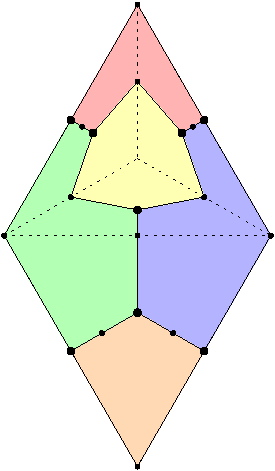
\includegraphics[align=c,height=3.2753cm]{../Thesis/Resources/Transformation-Algorithm-4.pdf}
  \end{figure}
\end{frame}

\subsection{Drawing the Polygonal Dual}
\label{subsect:drawing-the-polygonal-dual}

\begin{frame}
  \frametitle{\nameref{subsect:drawing-the-polygonal-dual}}
  \begin{itemize}
    \item Force-directed graph drawing \begin{itemize}
      \item Air pressure
      \item Angular resolution
      \item Vertex-vertex repulsion
      \item Vertex-edge repulsion
    \end{itemize}
    \item Preserve edge crossing and combinatorial properties: ImPrEd (Simonetto \etal{})
  \end{itemize}
  \begin{figure}
    \includegraphics[width=4cm]{../Thesis/Resources/Drawing-Forces-AirPressure.pdf}
    \qquad
    \includegraphics[width=4cm]{../Thesis/Resources/Drawing-Forces-AngularResolution.pdf}
  \end{figure}
\end{frame}





\section{Visualizing Dynamic Input Graphs}
\label{sect:visualizing-dynamic-input-graphs}

\begin{frame}
  \frametitle{Agenda}
  \begin{itemize}
    \item \light{\nameref{sect:introduction}}
    \item \light{\nameref{sect:visualizing-static-input-graphs}}
    \item \nameref{sect:visualizing-dynamic-input-graphs} \begin{itemize}
      \item \nameref{subsect:algorithmic-pipeline-dynamic}
      \item \nameref{subsect:incremental-transformation} \begin{itemize}
        \item \nameref{subsubsect:weight-changes}
        \item \nameref{subsubsect:inserting-vertices}
        \item \nameref{subsubsect:removing-vertices}
        \item \nameref{subsubsect:flipping-edges}
      \end{itemize}
    \end{itemize}
    \item \light{\nameref{sect:evaluation}}
  \end{itemize}
\end{frame}

\subsection{Algorithmic Pipeline}
\label{subsect:algorithmic-pipeline-dynamic}

\begin{frame}[c]
  \frametitle{\nameref{subsect:algorithmic-pipeline-static}}
  \begin{figure}
    \includegraphics[width=\textwidth]{../Thesis/Resources/Framework-3.pdf}
  \end{figure}
\end{frame}

\subsection{Incremental Transformation}
\label{subsect:incremental-transformation}

\subsubsection{Weight Changes}
\label{subsubsect:weight-changes}

\subsubsection{Inserting Vertices}
\label{subsubsect:inserting-vertices}

\begin{frame}
  \frametitle{\nameref{subsect:incremental-transformation}}
  \framesubtitle{Inserting Vertices}
  \begin{itemize}
    \item Internal faces in primal are triangles
    \item No preconditions
    \item Idea: insert new face in dual at point where three existing faces meet
  \end{itemize}
  \begin{figure}
    \includegraphics[height=2cm]{../Thesis/Resources/InsertVertex-Example-Inside-1.pdf}
    \quad
    \includegraphics[height=2cm]{../Thesis/Resources/InsertVertex-Example-Inside-2.pdf}
    \quad
    \includegraphics[height=2cm]{../Thesis/Resources/InsertVertex-Example-Inside-3.pdf}
    \quad
    \includegraphics[height=2cm]{../Thesis/Resources/InsertVertex-Example-Inside-4.pdf}
  \end{figure}
\end{frame}

\begin{frame}[c]
  \frametitle{\nameref{subsect:incremental-transformation}}
  \framesubtitle{Inserting Vertices \emdash{} Construction}
  \begin{figure}
    \includegraphics[height=2.7cm]{../Thesis/Resources/InsertVertex-Illustration-1.pdf}\quad
    \includegraphics[height=2.7cm]{../Thesis/Resources/InsertVertex-Illustration-2.pdf}\quad
    \includegraphics[height=2.7cm]{../Thesis/Resources/InsertVertex-Illustration-3.pdf}
  \end{figure}
\end{frame}

\begin{frame}[c]
  \frametitle{\nameref{subsect:incremental-transformation}}
  \framesubtitle{Inserting Vertices \emdash{} Implicit Outer Face}
  \begin{figure}
    \includegraphics[height=2.5cm]{../Thesis/Resources/InsertVertex-Duality-1.pdf}
    \quad
    \includegraphics[height=2.5cm]{../Thesis/Resources/InsertVertex-Duality-2.pdf}
  \end{figure}
  \begin{figure}
    \includegraphics[height=2.5cm]{../Thesis/Resources/InsertVertex-Duality-3.pdf}
    \qquad\qquad
    \includegraphics[height=2.5cm]{../Thesis/Resources/InsertVertex-Duality-4.pdf}
  \end{figure}
\end{frame}

\subsubsection{Removing Vertices}
\label{subsubsect:removing-vertices}

\begin{frame}
  \frametitle{\nameref{subsect:incremental-transformation}}
  \framesubtitle{Removing Vertices}
  \begin{itemize}
    \item Primal must remain internally triangulated
    \item Vertex to be removed must have degree 3
    \item Idea: remove boundary with one adjacent region
  \end{itemize}
  \begin{figure}
    \includegraphics[height=2cm]{../Thesis/Resources/RemoveVertex-Example-Internal-1.pdf}
    \quad
    \includegraphics[height=2cm]{../Thesis/Resources/RemoveVertex-Example-Internal-2.pdf}
    \quad
    \includegraphics[height=2cm]{../Thesis/Resources/RemoveVertex-Example-Internal-3.pdf}
    \quad
    \includegraphics[height=2cm]{../Thesis/Resources/RemoveVertex-Example-Internal-4.pdf}
  \end{figure}
\end{frame}

\begin{frame}[c]
  \frametitle{\nameref{subsect:incremental-transformation}}
  \framesubtitle{Removing Vertices \emdash{} Construction}
  \begin{figure}
    \includegraphics[height=4cm]{../Thesis/Resources/RemoveVertex-Illustration-1.pdf}
    \qquad
    \includegraphics[height=4cm]{../Thesis/Resources/RemoveVertex-Illustration-2.pdf}
  \end{figure}
\end{frame}

\subsubsection{Flipping Edges}
\label{subsubsect:flipping-edges}

\begin{frame}
  \frametitle{\nameref{subsect:incremental-transformation}}
  \framesubtitle{Flipping Edges}
  \begin{itemize}
    \item Internal edge is incident to two triangular faces
    \item Edge can only be flipped if vertices on either side aren’t already adjacent
    \item Idea \begin{itemize}
      \item Contact boundary to be removed into single point
      \item Create boundary in opposing direction
    \end{itemize}
  \end{itemize}
  \begin{figure}
    \includegraphics[height=2cm]{../Thesis/Resources/FlipEdge-Example-Internal-1.pdf}
    \quad
    \includegraphics[height=2cm]{../Thesis/Resources/FlipEdge-Example-Internal-2.pdf}
    \quad
    \includegraphics[height=2cm]{../Thesis/Resources/FlipEdge-Example-Internal-3.pdf}
    \quad
    \includegraphics[height=2cm]{../Thesis/Resources/FlipEdge-Example-Internal-4.pdf}
  \end{figure}
\end{frame}

\begin{frame}[c]
  \frametitle{\nameref{subsect:incremental-transformation}}
  \framesubtitle{Flipping Edges \emdash{} Construction \emdash{} Contract $u$-$v$-Boundary}
  \begin{figure}
    \includegraphics[width=3.25cm]{../Thesis/Resources/FlipEdge-ContractBoundaryBelow-1.pdf}
    \quad
    \includegraphics[width=3.25cm]{../Thesis/Resources/FlipEdge-ContractBoundaryBelow-2.pdf}
    \quad
    \includegraphics[width=3.25cm]{../Thesis/Resources/FlipEdge-ContractBoundaryBelow-3.pdf}
  \end{figure}
\end{frame}

\begin{frame}[c]
  \frametitle{\nameref{subsect:incremental-transformation}}
  \framesubtitle{Flipping Edges \emdash{} Construction \emdash{} Contract $u$-$v$-Boundary}
  \begin{figure}
    \includegraphics[width=3.25cm]{../Thesis/Resources/FlipEdge-ContractBoundaryAbove-1.pdf}
    \quad
    \includegraphics[width=3.25cm]{../Thesis/Resources/FlipEdge-ContractBoundaryAbove-2.pdf}
    \quad
    \includegraphics[width=3.25cm]{../Thesis/Resources/FlipEdge-ContractBoundaryAbove-3.pdf}
  \end{figure}
\end{frame}

\begin{frame}[c]
  \frametitle{\nameref{subsect:incremental-transformation}}
  \framesubtitle{Flipping Edges \emdash{} Construction \emdash{} Create $x$-$y$-Boundary}
  \begin{figure}
    \includegraphics[width=3.25cm]{../Thesis/Resources/FlipEdge-StretchBoundary-1.pdf}
    \quad
    \includegraphics[width=3.25cm]{../Thesis/Resources/FlipEdge-StretchBoundary-2.pdf}
    \quad
    \includegraphics[width=3.25cm]{../Thesis/Resources/FlipEdge-StretchBoundary-3.pdf}
  \end{figure}
\end{frame}

\begin{frame}[c]
  \frametitle{\nameref{subsect:incremental-transformation}}
  \framesubtitle{Flipping Edges \emdash{} Inserting and Removing Edges}
  \begin{figure}
    \includegraphics[height=2cm]{../Thesis/Resources/FlipEdge-Example-Insert-1.pdf}
    \quad
    \includegraphics[height=2cm]{../Thesis/Resources/FlipEdge-Example-Insert-2.pdf}
    \quad
    \includegraphics[height=2cm]{../Thesis/Resources/FlipEdge-Example-Insert-3.pdf}
    \quad
    \includegraphics[height=2cm]{../Thesis/Resources/FlipEdge-Example-Insert-4.pdf}
  \end{figure}
  \begin{figure}
    \includegraphics[height=2cm]{../Thesis/Resources/FlipEdge-Example-Remove-1.pdf}
    \quad
    \includegraphics[height=2cm]{../Thesis/Resources/FlipEdge-Example-Remove-2.pdf}
    \quad
    \includegraphics[height=2cm]{../Thesis/Resources/FlipEdge-Example-Remove-3.pdf}
    \quad
    \includegraphics[height=2cm]{../Thesis/Resources/FlipEdge-Example-Remove-4.pdf}
  \end{figure}
\end{frame}





\section{Evaluation}
\label{sect:evaluation}

\begin{frame}
  \frametitle{Agenda}
  \begin{itemize}
    \item \light{\nameref{sect:introduction}}
    \item \light{\nameref{sect:visualizing-static-input-graphs}}
    \item \light{\nameref{sect:visualizing-dynamic-input-graphs}}
    \item \nameref{sect:evaluation} \begin{itemize}
      \item \nameref{subsect:research-questions}
      \item \nameref{subsect:quality-metrics}
      \item \nameref{subsect:evaluation-results}
      \item \nameref{subsect:examples}
    \end{itemize}
  \end{itemize}
\end{frame}

\subsection{Research Questions}
\label{subsect:research-questions}

\begin{frame}
  \frametitle{\nameref{subsect:research-questions}}
  \begin{enumerate}
    \item Which quantitative measures best capture the quality of the maps generated by our algorithm in terms of \begin{itemize}
      \item accuracy?
      \item our understanding of locally fat regions?
    \end{itemize}
    \item What is the quality of the maps generated by our algorithm according to these quality metrics? \begin{itemize}
      \item How does this quality change based on the size and other properties of the input graph? 
      \item How does this quality change over time as dynamic updates are incorporated? 
    \end{itemize}
  \end{enumerate}
\end{frame}

\subsection{Quality Metrics}
\label{subsect:quality-metrics}

\begin{frame}
  \frametitle{\nameref{subsect:quality-metrics}}
  \begin{itemize}
    \item Cartographic error \begin{itemize}
      \item How much do the actual region areas differ from the prescribed ones?
    \end{itemize}
    \item Polygon complexity \begin{itemize}
      \item How convex is the polygon?
      \item What's the frequency and amplitude of the ``vibration" on the polygon's boundary?
% Example: circle vs star
    \end{itemize}
  \end{itemize}
\end{frame}

\subsection{Evaluation Results}
\label{subsect:evaluation-results}

\begin{frame}[c]
  \frametitle{\nameref{subsect:evaluation-results}}
  \framesubtitle{Effect of initial number of clusters}
  \begin{figure}
    \includegraphics[width=5cm]{../Thesis/Resources/Evaluation-AverageCartographicError-n.pdf}
    \quad
    \includegraphics[width=5cm]{../Thesis/Resources/Evaluation-AveragePolygonComplexity-n.pdf}
  \end{figure}
\end{frame}

\begin{frame}[c]
  \frametitle{\nameref{subsect:evaluation-results}}
  \framesubtitle{Effect of number of operations}
  \begin{figure}
    \includegraphics[width=5cm]{../Thesis/Resources/Evaluation-AverageCartographicError-t.pdf}
    \quad
    \includegraphics[width=5cm]{../Thesis/Resources/Evaluation-AveragePolygonComplexity-t.pdf}
  \end{figure}
\end{frame}

\subsection{Examples}
\label{subsect:examples}

\begin{frame}[c]
  \frametitle{\nameref{subsect:examples}}
  \framesubtitle{Maps with $n$ = 10}
  \begin{figure}
    \includegraphics[width=5cm]{../Thesis/Resources/Evaluation-Example-n10-0F69CDD9-EAAD-4F81-934F-8BA98B1424F6-2.pdf}
    \quad
    \includegraphics[width=5cm]{../Thesis/Resources/Evaluation-Example-n10-9A841901-DFA0-4ECD-A758-87E1C8A1D0D0-0.pdf}
  \end{figure}
\end{frame}

\begin{frame}[c]
  \frametitle{\nameref{subsect:examples}}
  \framesubtitle{Maps with $n$ = 20}
  \begin{figure}
    \includegraphics[width=5cm]{../Thesis/Resources/Evaluation-Example-n20-450053F2-5F0A-4CFE-8A08-92CC201A07B9-0.pdf}
    \quad
    \includegraphics[width=5cm]{../Thesis/Resources/Evaluation-Example-n20-AE097F3A-14FD-4735-A19B-8FD343CA3346-0.pdf}
  \end{figure}
\end{frame}

\begin{frame}[c]
  \frametitle{\nameref{subsect:examples}}
  \framesubtitle{Maps with $n$ = 30}
  \begin{figure}
    \includegraphics[width=5cm]{../Thesis/Resources/Evaluation-Example-n30-9BA67779-50C2-483B-8E81-916125D5D3F7-0.pdf}
    \quad
    \includegraphics[width=5cm]{../Thesis/Resources/Evaluation-Example-n30-45D8EAD2-210C-4F04-8C7F-EA3E65484875-0.pdf}
  \end{figure}
\end{frame}





\end{document}
